Como hemos visto anteriormente, el histograma de los logaritmos de las ejecuciones parece tener múltiples picos, podría sugerir que sus datos son una mezcla de varias distribuciones normales.

Una forma de modelar este tipo de datos es utilizar un modelo mixto, que supone que los datos se generan mediante una combinación de varias distribuciones subyacentes. En su caso, podría usar un modelo de mezcla gaussiana para representar sus datos como una mezcla de varias distribuciones normales.

Una vez que ajustado un modelo de mezcla gaussiana a los datos, podría usarse para varios propósitos, como:

\begin{itemize}
    \item Clustering: El modelo puede utilizarse para agrupar los datos en diferentes grupos (clusters) en función de su similitud. Cada componente gaussiana del modelo representa un grupo diferente y los datos se asignan al grupo cuya componente gaussiana tenga la mayor probabilidad.

    \item Detección de valores atípicos: El modelo puede utilizarse para detectar valores atípicos en los datos. Los valores atípicos son aquellos puntos que tienen una baja probabilidad según el modelo ajustado.

    \item Estimación de densidad: El modelo puede utilizarse para estimar la función de densidad subyacente de los datos. La función de densidad se puede utilizar para generar nuevos datos sintéticos o para calcular probabilidades.
\end{itemize}

Aunque este tema está fuera del alcance del curso, se realizó una aproximación a la técnica cuyo resultado es el mostrado en la figura \ref{figure:gaussmix}.

\begin{figure}[h]
    \begin{center}
        \scalebox{0.7}{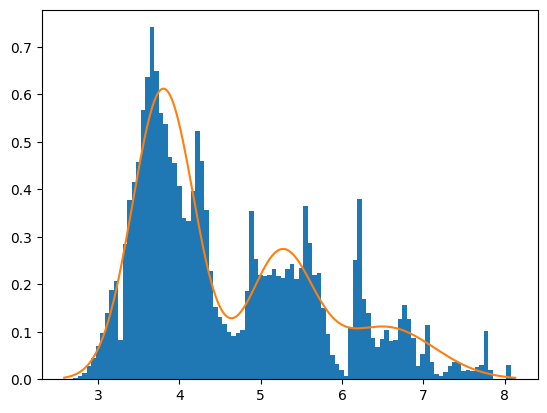
\includegraphics{gaussmix.png}}
    \end{center}
    \caption{\label{figure:gaussmix}Histograma del logaritmo de los tiempos de ejecución y modelo de mezcla gaussiana ajustado con 3 componentes. El eje x representa el logaritmo del tiempo de ejecución en milisegundos, mientras que el eje y representa la densidad.}
\end{figure}